%!TEX root = forallxbris.tex
\part{Interpretations}
\label{ch.semantics}
\addtocontents{toc}{\protect\mbox{}\protect\hrulefill\par}


\chapter{Extensionality}\label{s:Interpretations}

Recall that TFL is a truth-functional language. Its connectives are all truth-functional, and \emph{all} that we can do with TFL is key sentences to particular truth values. We can do this \emph{directly}. For example, we might stipulate that the TFL sentence $P$ is to be true. Alternatively, we can do this \emph{indirectly}, offering a symbolization key, e.g.:
	\begin{ekey}
		\item[P] Big Ben is in London
	\end{ekey}
Now recall from \S\ref{s:TruthFunctionality} that this should be taken to mean:
	\begin{ebullet}
		\item The TFL sentence $P$ is to take the same truth value as the English sentence `Big Ben is in London' (whatever that truth value may be)
	\end{ebullet}
The point that we emphasized is that TFL cannot handle differences in meaning that go beyond mere differences in truth value.


\section{Symbolizing versus translating}
FOL has some similar limitations, but it goes beyond mere truth values, since it enables us to split up sentences into terms, predicates and quantifier expressions. This enables us to consider what is \emph{true of} some particular object, or of some or all objects. But we can do no more than that.

When we provide a symbolization key for some FOL predicates, such as:
	\begin{ekey}
		\item[Cx] \gap{x} teaches Logic III in Calgary
	\end{ekey}
we do not carry the \emph{meaning} of the English predicate across into our FOL predicate. We are simply stipulating something like the following:
	\begin{ebullet}
		\item $Cx$ and `\gap{x} teaches Logic III in Calgary' are to be \emph{true of} exactly the same things.
	\end{ebullet}
So, in particular:
	\begin{ebullet}
		\item $Cx$ is to be true of all and only those things which teach Logic III in Calgary (whatever those things might be).
	\end{ebullet}
This is an indirect stipulation. Alternatively, we can directly stipulate which objects a predicate should be true of. For example, we can stipulate that $Cx$ is to be true of Richard Zach, and Richard Zach alone. As it happens, this direct stipulation would have the same effect as the indirect stipulation. Note, however, that the English predicates `\blank\ is Richard Zach' and `\blank\ teaches Logic III in Calgary' have very different meanings!

The point is that FOL does not give us any resources for dealing with nuances of meaning. When we interpret FOL, all we are considering is what the predicates are true of, regardless of whether we specify these things directly or indirectly. The things a predicate is true of are known as the \define{extension} of that predicate. We say that FOL is an \define{extensional language} because FOL does not represent differences of meaning between predicates that have the same extension.

For this reason, we say only that FOL sentences \emph{symbolize} English sentences. It is doubtful that we are \emph{translating} English into FOL, as translations should preserve meanings, and not just extensions.

\section{A word on extensions}
We can stipulate directly what predicates are to be true of, so it is worth noting that our stipulations can be as arbitrary as we like. For example, we could stipulate that $Hx$ should be true of, and only of, the following objects:
	\begin{center}
		Justin Trudeau\\
		the number $\pi$\\
		every top-F key on every piano ever made
	\end{center}
Now, the objects that we have listed have nothing particularly in common. But this doesn't matter. Logic doesn't care about what strikes us mere humans as `natural' or `similar'. Armed with this interpretation of $Hx$, suppose we now add to our symbolization key:
	\begin{ekey}
		\item[j] Justin Trudeau
		\item[r] Rachel Notley
		\item[p] the number $\pi$
	\end{ekey}
Then $Hj$ and $Hp$ will both be true, on this interpretation, but $Hr$ will be false, since Rachel Notley was not among the stipulated objects.



\section{Many-place predicates}
All of this is quite easy to understand when it comes to one-place predicates, but it gets messier when we consider two-place predicates. Consider a symbolization key like:
	\begin{ekey}
		\item[Lxy] \gap{x} loves \gap{y}
	\end{ekey}
Given what we said above, this symbolization key should be read as saying:
	\begin{earg}
		\item[\textbullet] $Lxy$ and `\gap{x} loves \gap{y}' are to be true of exactly the same things
	\end{earg}
So, in particular:
	\begin{earg}
		\item[\textbullet] $Lxy$ is to be true of x and y (in that order) iff x loves y.
	\end{earg}
It is important that we insist upon the order here, since love---famously---is not always reciprocated. (Note that `x' and `y' here are symbols of augmented English, and that they are being \emph{used}. By contrast, $x$ and $y$ are symbols of FOL, and they are being \emph{mentioned}.)

That is an indirect stipulation. What about a direct stipulation? This is slightly harder. If we \emph{simply} list objects that fall under $Lxy$, we will not know whether they are the lover or the beloved (or both). We have to find a way to include the order in our explicit stipulation.

To do this, we can specify that two-place predicates are true of \emph{pairs} of objects, where the order of the pair is important. Thus we might stipulate that $Bxy$ is to be true of, and only of, the following pairs of objects:
	\begin{center}
		\ntuple{Lenin, Marx}\\
		\ntuple{Heidegger, Sartre}\\
		\ntuple{Sartre, Heidegger}
	\end{center}
Here the angle-brackets keep us informed concerning order. Suppose we now add the following stipulations:
	\begin{ekey}
		\item[l] Lenin
		\item[m] Marx
		\item[h] Heidegger
		\item[r] Sartre
	\end{ekey}
Then $Blm$ will be true, since \ntuple{Lenin, Marx} was in our explicit list, but $Bml$ will be false, since \ntuple{Marx, Lenin} was not in our list. However, both $Bhr$ and $Brh$ will be true, since both \ntuple{Heidegger, Sartre} and \ntuple{Sartre, Heidegger} are in our explicit list.

To make these ideas more precise, we would need to develop some \emph{set theory}. That would give us some precise tools for dealing with extensions and with ordered pairs (and ordered triples, etc.). However, set theory is not covered in this book, so we will leave these ideas at an imprecise level. Nevertheless, the general idea should be clear.




\section{Interpretation}
We defined a \define{valuation} in TFL as any assignment of truth and falsity to atomic sentences. In FOL, we are going to define an \define{interpretation} as consisting of three things:
	\begin{ebullet}
		\item the specification of a domain
		\item for each name that we care to consider, an assignment of exactly one object within the domain
		\item for each predicate that we care to consider, a specification of what things (in what order) the predicate is to be true of
	\end{ebullet}
The symbolization keys that we considered in Part~\ref{ch.FOL} consequently give us one very convenient way to present an interpretation. We will continue to use them throughout this chapter. However, it is sometimes also convenient to present an interpretation \emph{diagrammatically}.

\newglossaryentry{interpretation}{
  name = {interpretation},
  description = {a specification of a \gls{domain} together with the objects the \glspl{name} pick out and which objects the \glspl{predicate} are true of}
}

Suppose we want to consider just a single two-place predicate, $Rxy$. Then we can represent it just by drawing an arrow between two objects, and stipulate that $Rxy$ is to hold of x and y just in case there is an arrow running from x to y in our diagram. As an example, we might offer:
\begin{center}
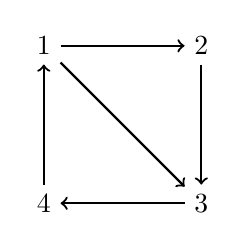
\begin{tikzpicture}
\node (atom1) at (0,2) {1};
\node (atom2) at (2,2) {2};
\node (atom3) at (2,0) {3};
\node (atom4) at (0,0) {4};
\draw[->, thick] (atom1)--(atom2);
\draw[->, thick] (atom2)--(atom3);
\draw[->, thick] (atom3)--(atom4);
\draw[->, thick] (atom4)--(atom1);
\draw[->, thick] (atom1) -- (atom3);
\end{tikzpicture}
\end{center}
This would be suitable to characterize an interpretation whose domain is the first four positive whole numbers, and which interprets $Rxy$ as being true of and only of:
	\begin{center}
		\ntuple{1, 2},
		\ntuple{2, 3},
		\ntuple{3, 4},
		\ntuple{4, 1},
		\ntuple{1, 3}
	\end{center}
Equally we might offer:

\begin{center}
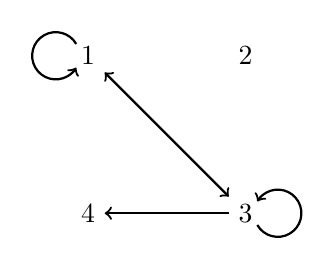
\begin{tikzpicture}
\node (atom1) at (0,2) {1};
\node (atom2) at (2,2) {2};
\node (atom3) at (2,0) {3};
\node (atom4) at (0,0) {4};
\draw[->, thick] (atom3)--(atom4);
\draw[->, thick] (atom1)+(-0.15,0.15) arc (-330:-30:.3);
\draw[->, thick] (atom3)+(0.15,-0.15) arc (-150:150:.3);
\draw[<->, thick] (atom1) -- (atom3);
\end{tikzpicture}
\end{center}
for an interpretation with the same domain, which interprets $Rxy$ as being true of and only of:
	\begin{center}
		\ntuple{1, 3},
		\ntuple{3, 1},
		\ntuple{3, 4},
		\ntuple{1, 1},
		\ntuple{3, 3}
	\end{center}
If we wanted, we could make our diagrams more complex. For example, we could add names as labels for particular objects. Equally, to symbolize the extension of a one-place predicate, we might simply draw a ring around some particular objects and stipulate that the thus encircled objects (and only them) are to fall under the predicate $Hx$, say.


\chapter{Truth in FOL}\label{s:TruthFOL}
We know what interpretations are. Since, among other things, they tell us which predicates are true of which objects, they will provide us with an account of the truth of atomic sentences. However, we must also present a detailed account of what it is for an arbitrary FOL sentence to be true or false in an interpretation.

But we defined what a sentence was by first specifying what a formula is. Formulas like $Hx$ aren't the sorts of things that are true or false in interpretations. Only sentences are true or false. But if we provide extra information we can determine the truth of $Hx$: we need to specify what $x$ refers to. This is done by using a variable assignment: \factoidbox{A variable assignment specifies an object for each variable.}

We define whether a formula is true or false \emph{under a variable assignment}.
We know from \S\ref{s:FOLSentences} that there are three kinds of formulas in FOL:
	\begin{ebullet}
		\item atomic formulas
		\item formulas whose main logical operator is a sentential connective
		\item formulas whose main logical operator is a quantifier
	\end{ebullet}
We need to explain truth for all three kinds of formula.

We will provide a completely general explanation in this section. However, to try to keep the explanation comprehensible, we will, at several points, use the following interpretation:
	\begin{ekey}
		\item[\text{domain}] all people born before 2000\textsc{ce}
		\item[a] Aristotle
		\item[b] Beyonc\'e
		\item[Px] \gap{x} is a philosopher
		\item[Rxy] \gap{x} was born before \gap{y}
	\end{ekey}
This will be our \emph{go-to example} in what follows.

\section{Atomic formulas}
Atomic formulas are things like $Px$, $Pb$ or $Rax$.

An atomic sentence like $Pb$ is checked for truth just by consulting our interpretation: $Px$ is `\gap{x} is a philosopher', so if we're looking at $Pb$ we fill out the gap with  Beyonc\'e, and  Beyonc\'e is not a philosopher, so $Pb$ is false.

What about $Px$? This reads something like `they are a philosopher'. The question is who `they' refers to, or in the logic terms: who $x$ is. This depends on a variable assignment. Our variable assignment needs to give an object in our domain for the variable $x$. For example, it might give Beyonc\'e, then since Beyonc\'e is not a philosopher, $Px$ would be false on this variable assignment. Our variable assignment doesn't need to specify one of the objects that are named, it can give us anyone in our domain, e.g.~Queen Elizabeth II. Under the variable assignment which assigns $x$ Queen Elizabeth II, $Px$ is false: Queen Elizabeth II is not a philosopher.

%The truth of atomic \emph{sentences} should be fairly straightforward. The sentence $Pa$ should be true just in case $Px$ is true of $a$. Given our go-to interpretation, this is true iff Aristotle is a philosopher. Aristotle is a philosopher. So the sentence is true. Equally, $Pb$ is false on our go-to interpretation.

Likewise, on this interpretation, $Rab$ is true iff the object named by $a$ was born before the object named by $b$. Well, Aristotle was born before Beyonc\'e. So $Rab$ is true. Equally, $Raa$ is false: Aristotle was not born before Aristotle. How about $Rax$? Well what does our variable assignment specify for $x$? If we have a variable assignment where $x$ is Queen Elizabeth II, then $Rax$ is true: Aristotle was born before Queen Elizabeth II.

Dealing with atomic sentences, then, is very intuitive. When \meta{R} is an $n$-place predicate and $\metaterm_1,\,\metaterm_2\ldots\metaterm_{n}$ are names or variables, then

	\factoidbox{
		$\meta{R}\metaterm_1\metaterm_2\ldots\metaterm_{n}$ is true in an interpretation under a variable assignment \textbf{iff}\\
		$\meta{R}$ is true of the objects referred to by $\metaterm_{1}, \metaterm_{2}, \ldots, \metaterm_{n}$ in that interpretation under that variable assignment (considered in that order)
	}



\section{Sentential connectives}
We saw in \S\ref{s:FOLSentences} that FOL formulas can be built up from simpler ones using the truth-functional connectives that were familiar from TFL. The rules governing these truth-functional connectives are \emph{exactly} the same as they were when we considered TFL. Here they are:
	\factoidbox{
		$\metaX \eand \metaY$ is true in an interpretation under a variable assignment \textbf{iff}\\ both $\metaX$ and $\metaY$ is true in that interpretation under that variable assignment

		\
		\\
		$\metaX \eor \metaY$ is true in an interpretation under a variable assignment \textbf{iff}\\ either $\metaX$ is true or $\metaY$ is true in that interpretation under that variable assignment

		\
		\\$\enot \metaX$ is true in an interpretation under a variable assignment \textbf{iff} \\$\metaX$ is false in that interpretation under that variable assignment

		\
		\\$\metaX \eif \metaY$ is true in an interpretation under a variable assignment \textbf{iff}\\ either $\metaX$ is false or $\metaY$ is true in that interpretation under that variable assignment

		\
		\\$\metaX \eiff \metaY$ is true in an interpretation under a variable assignment \textbf{iff} \\$\metaX$ has the same truth value as $\metaY$ in that interpretation under that variable assignment
	}
This is just another presentation of the truth rules we gave for the connectives in TFL; it just does so in a slightly different way. Some examples will probably help to illustrate the idea. On our go-to interpretation:
	\begin{earg}
		\item[\textbullet] $ Pa$ is true
		\item[\textbullet] $Rab \eand Pb$ is false because, although $Rab$ is true, $Pb$ is false
		\item[\textbullet] $\enot Pa$ is false
		\item[\textbullet] $Pa \eand \enot(Pb\eand Rab)$ is true, because $Pa$ is true and $Pb$ is false, so $Pb\eand Rab$ is false, thus $\enot (Pb\eand Rab)$ is also true.
	\end{earg}
Make sure you understand these examples.

We can also carry variable assignments around with us. Consider a variable assignment which assigns David Hume to $x$. Then \begin{ebullet}
\item $Px$ is true under this variable assignment: David Hume was a philosopher
\item $Bxa$ is false under this variable assignment: David Hume was born after Aristotle
\item $Px\eif Bxa$ is false under this variable assignment: $Px$ is true and $Bxa$ is false, so by our rule for $\eif$, $Px\eif Bxa$ is false.
\end{ebullet}


\section{When the main logical operator is a quantifier}
The exciting innovation in FOL, though, is the use of \emph{quantifiers}.

Consider the following interpretation:
\begin{center}
\begin{tikzpicture}
\node (A) [alice,monitor,sword,minimum size=1cm] {Alice};
\node (B)[bob,evil,sword,minimum size=1cm,right=1cm of A] {Bob};
\node[charlie,monitor,female, minimum size=1cm,below=.8cm of A] {Cathy};
\node[businessman,minimum size=1cm,skin=brown,below=.8cm of B] {Denny};
\end{tikzpicture}

\begin{ekey}\item[\text{domain}] People in above picture (Alice, Bob, Cathy and Denny)
\item[Hx] \gap{x} has horns (Bob)
\item[Sx] \gap{x} carrying a sword (Alice and Bob)
\item[Cx]\gap{x} is looking at a computer (Alice and Cathy)
%\item[Gx] nothing
\end{ekey}
\end{center}

Is $\exists x Sx$ true? To check this we see if there is a choice of an object for $x$ which gives us a variable assignment under which $Sx$ is true. Consider assigning Alice to $x$, which we can as shorthand write by $x\mapsto \text{Alice}$. Under this variable assignment, $Sx$ is true: Alice does have a sword. So $\exists x Sx$ is true. There is a choice of an object in our domain for $x$ under which $Sx$ is true.

What about $\forall x Sx$? This is true iff $Sx$ is true under any choice of a person for $x$. Let's go through them. \begin{center}
\begin{tabular}{l|c}
&$Sx$\Bstrut\\\hline\Tstrut
$x\mapsto\text{Alice}$&T\\
$x\mapsto \text{Bob}$&T\\
$x\mapsto \text{Cathy}$&F\\
$x\mapsto \text{Denny}$&F
\end{tabular}
\end{center}So $\forall x Sx$ is false: it is not the case that $Sx$ is true under any choice of an object for $x$: when we have an assignment of Cathy to $x$, $Sx$ is false.

What about $\forall x(Sx\eif (Hx\eor Cx))$
\begin{center}
\begin{tabular}{l|ccccc}
&$Sx$&$Hx$&$Cx$&$Hx\eor Cx$&$Sx\eif (Hx\eor Cx)$\Bstrut\\\hline\Tstrut
$x\mapsto\text{Alice}$&T&F&T&T&T\\
$x\mapsto \text{Bob}$&T&T&F&T&T\\
$x\mapsto \text{Cathy}$&F&F&T&T&T\\
$x\mapsto \text{Denny}$&F&F&F&F&T
\end{tabular}
\end{center}
So $Sx\eif (Hx\eor Cx)$  is true under every assignment of an object to the variable $x$. And so $\forall x(Sx\eif (Hx\eor Cx))$ is true.



We have to tread more carefully once we start having multiple quantifiers. Let's walk through some cases.

Consider a new interpretation: \begin{center}
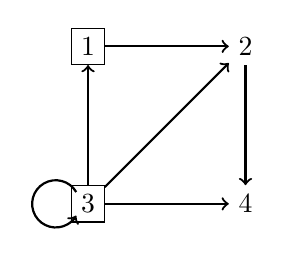
\begin{tikzpicture}
\node (atom1) [draw] at (0,2) {1};
\node (atom2) at (2,2) {2};
\node (atom3) [draw] at (0,0) {3};
\node (atom4)  at (2,0) {4};
\draw[->, thick] (atom3)+(-0.15,0.15) arc (-330:-30:.3);
\draw[<-, thick] (atom2) -- (atom3);
\draw[<-,thick] (atom1)--(atom3);
\draw[<-, thick] (atom4)--(atom3);
\draw[->, thick] (atom1)--(atom2);
\draw[->, thick] (atom2)--(atom4);
\end{tikzpicture}

 \begin{ekey}
\item[\text{domain}] Numbers 1, 2, 3 and 4.
\item[Rxy] There is an arrow from \gap{x} to \gap{y} in the diagram.
\item[Sx] There is a square around \gap{x} in the diagram.
\end{ekey}
\end{center}

 Is $\exists x\forall y Rxy$ true? We need to find some choice of an object for $x$ where $\forall y Rxy$ is true under that choice (``variable assignment''). Let's (with foresight) chose the number 3 for $x$ ($x\mapsto 3$). Is $\forall y Rxy$ true under this variable assignment $x\mapsto 3$? To check this we need to do something more with our variable assignment: we need to extend it with a choice of an object for $y$. Moreover, we need to think about all ways of picking an object for $y$, while we've fixed $x$ as the number 3. Consider, e.g.~$y\mapsto 1$. Then we have to evaluate whether $Rxy$ is true with $x\mapsto 3,\, y\mapsto 1$. This is true iff there is an arrow from 3 ($x$) to 1 ($y$), and there is such an arrow.  We can work through all the cases an see that all of them have an arrow from $3$, so $Rxy$ is true for any choice of object for $y$:
\begin{center}
 \begin{tabular}{cc|c}
&&$Rxy$\Bstrut\\\hline\Tstrut
$x\mapsto 3$&$y\mapsto 1$&T\\
$x\mapsto 3$&$y\mapsto 2$&T\\
$x\mapsto 3$&$y\mapsto 3$&T\\
$x\mapsto 3$&$y\mapsto 4$&T\\
 \end{tabular}
\end{center}So under any way of extending our variable assignment of $x\mapsto 3$ by choosing an object for $y$ results in a variable assignment on which $Rxy$ true. This tells us that $\forall y Rxy$ is true under the variable assignment $x\mapsto 3$. And \emph{that} tells us that $\exists x\forall y Rxy$ is true: there's an assignment of the variable $x$ under which the constituent formula $\forall y Rxy$ is true.

What about $\exists x \exists y(Rxy \eand Ryx)$? To show that it is true we will want to choose an object that we can assign to $x$ under which $\exists y (Rxy\eand Ryx)$ is true. Let's consider $x\mapsto 3$ (again I'm using my forsight of what will come to choose carefully). Now is $\exists y (Rxy\eand Ryx)$  true under the variable assignment $x\mapsto 3$? We need to find an extension of this which chooses an object for $y$ under which $Rxy\eand Ryx$ is true. Consider $y\mapsto 3$. We now have a variable assignment $x\mapsto 3, y\mapsto 3$. They are different variables but there's nothing stopping them denoting the same object. And we can then consider whether $Rxy\eand Ryx$ is true under this interpretation. Well, $Rxy$ is true: 3 does have an arrow to 3. And $Ryx$ is also true: 3 does have an arrow to 3. So by our clause for $\eand$, $Rxy\eand Ryx$ is true under this variable assignment $x\mapsto 3, y\mapsto 3$. And so $\exists y(Rxy\eand Ryx)$ is true under the variable assignment $x\mapsto 3$. And so $\exists x\exists y(Rxy\eand Ryx)$ is true in this interpretation.

One more example: $\forall x(Sx\eif \exists y Rxy)$? To check this is true we will need to go through each of our objects for $x$ and see that $Sx\eif \exists y Rxy$ is true under that interpretation. We can already see if $Sx$ is true under each variable assignment, and if we find that $Sx$ is false that's enough information to determine that $Sx\eif \exists y Rxy$ is true (check the definition of truth for $\eif$ to see this):
\begin{center}
\begin{tabular}{c|ccc}
&$Sx$&$\exists y Rxy$&$Sx\eif\exists y Rxy$\Bstrut\\\hline\Tstrut
$x\mapsto 1$&T&?&?\\
$x\mapsto 2$&F&?&T\\
$x\mapsto 3$&T&?&?\\
$x\mapsto 4$&F&?&T
\end{tabular}
\end{center}

So we need to check  whether $\exists y Rxy$ is true under the variable assignments $x\mapsto 1$ and $x\mapsto 3$.

Consider $x\mapsto 1$. We can find an object for $y$ where $Rxy$ is true under that variable assignment: consider $y\mapsto 2$. Since there is an arrow from 1 to 2, $Rxy$ is true in the variable assignment $x\mapsto 1$ and $y\mapsto 2$. Thus $\exists y Rxy$ is true on the variable assignment $x\mapsto 1$. We're also able to do something similar for $x\mapsto 3$:
\begin{center}
\begin{tabular}{cc|c}
&&$Rxy$\Bstrut\\\hline\Tstrut
$x\mapsto 1$&$y\mapsto 2$&T\\
$x\mapsto 3$&$y\mapsto 3$&T
 \end{tabular}
\end{center}So we now have
\begin{center}
\begin{tabular}{c|ccc}
&$Sx$&$\exists y Rxy$&$Sx\eif\exists y Rxy$\Bstrut\\\hline\Tstrut
$x\mapsto 1$&T&T&T\\
$x\mapsto 2$&F&?&T\\
$x\mapsto 3$&T&T&T\\
$x\mapsto 4$&F&?&T
\end{tabular}
\end{center}So $\forall x(Sx\eif \exists y Rxy)$ is true. Informally we might say this as: for every number that has a square around it has an arrow going out of it.

One final example: $\forall x\forall y Rxy$. To check this we will need to consider all choices for $x$ and all choices for $y$ and check $Rxy$ is true on all of them. There are 16 such choices. But we won't have to go through them all: it'll be false. Consider $x\mapsto 1$ and $y\mapsto 4$. $Rxy$ is false under this variable assignment: there is no arrow from 1 to 4. Thus $\forall yRxy$ is false on the variable assignment $x\mapsto 1$. And so $\forall x\forall y Rxy$ is false in the interpretation.

 Let's now give a formal definition of the idea we've been using here. Quantified formulas like $\exists y Rxy$ still need to be given truth conditions \emph{relative to a variable assignment}, because we'll need to specify an assignment of an object for the free variable $x$. So we define when $\exists \metav\metaX$ is true under a variable assignment $\alpha$, which might be, e.g.~$x\mapsto 1$. To give a general definition, though we might also consider whether $\forall y Rxy$ is true under a variable assignment $x\mapsto 1, y\mapsto 4$. This is slightly odd: we're considering $\exists y Rxy$ but have been told who $y$ refers to already. However when we evaluate it we simply ignore whatever our given variable assignment tells us about $y$: we consider variable assignments that modify the assignment by changing what is assigned to $y$. And by modifying it to $x\mapsto 1, y\mapsto2$ we have a variable assignment under which $Rxy$ is true, so $\exists y Rxy$ is true under the original variable assignment $x\mapsto 1, y\mapsto 4$.

 Similarly consider $\exists x Sx$ under the variable assignment $x\mapsto 1$. To evaluate this we consider modification of this variable assignment which assign other objects to $x$. Under the variable assignment $x\mapsto 2$, $Sx$ is true.  So under our original variable assignment $\exists x Sx$ is true: it didn't matter what our original variable assignment was, we ignored this and considered variants to evaluate its truth.

 This is a general feature: Sentences, which have all variables bound, have truth values independent of any variable assignment they're evaluated with: when we have a quantifier like $\exists x$ or $\forall x$ we ignore whatever our original variable assignment told us about $x$. So when all our variables are bound by quantifiers, all the original components of our variable assignment are ignored. To summarise: Sentences are simply true or false in interpretations, variable assignments don't matter.

 Now for our formal definition:
\factoidbox{
$\forall \metav\metaX$ is true under a variable assignment $\alpha$\\
\textbf{iff} $\metaX$ is true under \emph{every} variable assignment that is the result of modifying/extending $\alpha$ with a choice of an object in our domain for $\metav$.

\bigskip

$\exists \metav\metaX$ is true under a variable assignment $\alpha$\\
\textbf{iff} $\metaX$ is true under \emph{some} variable assignment that is the result of modifying/extending $\alpha$ with a choice of an object in our domain for $\metav$.
}
To be clear: all this is doing is formalizing the intuitive idea expressed in our examples. The result is a bit ugly, and the final definition might look a bit opaque. Hopefully, though, the \emph{spirit} of the idea is clear.


%\section{When the main logical operator is a quantifier}
%The exciting innovation in FOL, though, is the use of \emph{quantifiers}.
%%When is $\forall x Px$ true? The thought is: we introduce a new name: $d$, and we check if $Pd$ is true in the various interpretations where $d$ names the different objects.
%But expressing the truth conditions for quantified sentences is a bit more fiddly than one might first expect.
%
%Here is a na\"{i}ve first thought. We want to say that $\forall x Fx$ is true iff $Fx$ is true of everything in the domain. This should not be too problematic: our interpretation will specify directly what $Fx$ is true of.
%
%Unfortunately, this na\"{i}ve thought is not general enough. For example, we want to be able to say that $\forall x \exists y Lxy$ is true just in case $\exists y Lxy$ is true of everything in the domain. This is problematic, since our interpretation does not directly specify what $\exists y Lxy$ is to be true of. Instead, whether or not this is true of something should follow just from the interpretation of $Lxy$, the domain, and the meanings of the quantifiers.
%
%So here is a second na\"{i}ve thought. We might try to say that $\forall x \exists y Lxy$ is to be true in an interpretation iff $\exists y L\meta{a}y$ is true for \emph{every} name \meta{a} that we have included in our interpretation. Similarly, we might try to say that $\exists y L\meta{a}y$ is true just in case $L\meta{a}\meta{b}$ is true for \emph{some} name \meta{b} that we have included in our interpretation.
%
%Unfortunately, this is not right either. To see this, observe that in our go-to interpretation, we have only given interpretations for \emph{two} names, $a$ and $b$, but the domain---all people born before the year 2000\textsc{ce}---contains many more than two people. We have no intention of trying to name \emph{all} of them!
%
%So here is a third thought. (And this thought is not na\"{i}ve, but correct.) Although it is not the case that we have named \emph{everyone}, each person \emph{could} have been given a name. So we should focus on this possibility of extending an interpretation, by adding a new name. We will offer a few examples of how this might work, centring on our go-to interpretation, and we will then present the formal definition.
%
%In our go-to interpretation, $\exists x Rbx$ should be true. After all, in the domain, there is certainly someone who was born after Beyonc\'e. Lady Gaga is one of those people. Indeed, if we were to extend our go-to interpretation---temporarily, mind---by adding the name $c$ to refer to Lady Gaga, then $Rbc$ would be true on this extended interpretation. This, surely, should suffice to make $\exists x Rbx$ true on the original go-to interpretation.
%
%In our go-to interpretation, $\exists x (Px \eand Rxa)$ should also be true. After all, in the domain, there is certainly someone who was both a philosopher and born before Aristotle. Socrates is one such person. Indeed, if we were to extend our go-to interpretation by letting a new name, $c$, denote Socrates, then $Wc \eand Rca$ would be true on this extended interpretation. Again, this should surely suffice to make $\exists x (Px \eand Rxa)$ true on the original go-to interpretation.
%
%In our go-to interpretation, $\forall x \exists y Rxy$ should be false. After all, consider the last person born in the year 1999. We don't know who that was, but if we were to extend our go-to interpretation by letting a new name, $d$, denote that person, then we would not be able to find anyone else in the domain to denote with some further new name, perhaps $e$, in such a way that $Rde$ would be true. Indeed, no matter \emph{whom} we named with $e$, $Rde$ would be false. This observation is surely sufficient to make $\exists y Rdy$ \emph{false} in our extended interpretation, which in turn is surely sufficient to make $\forall x \exists y Rxy$ false on the original go-to interpretation.
%
%If you have understood these three examples, good. That's what matters. Strictly speaking, though, we still need to give a precise definition of the truth conditions for quantified sentences. The result, sadly, is a bit ugly, and requires a few new definitions. Brace yourself!
%
%Suppose that \metaX is an expression with that $\meta{x}$ is free in $\metaX$ (i.e.~no quantifiers $\forall\meta{x}$ or $\exists\meta{x}$ already). We will write this thus:
%$$\metaX(\ldots \meta{x} \ldots \meta{x} \ldots)$$
%Suppose also that \meta{c} is a name. Then we will write:
%$$\metaX(\ldots \meta{c} \ldots \meta{c} \ldots)$$
%for the formula obtained by replacing every occurrence of $\meta{x}$ in \metaX with $\meta{c}$. The resulting formula is called a \define{substitution instance} of $\forall \meta{x}\metaX$ and $\exists\meta{x}\metaX$.  $\meta{c}$ is called the \define{instantiating name}. So:
%	$$\exists x (Rex \eiff Fx)$$
%is a substitution instance of
%	$$\forall y \exists x (Ryx \eiff Fx)$$
%with the instantiating name $e$.
%
%\newglossaryentry{substitution instance}{
%  name = substitution instance,
%  description = {the result of replacing every occurrence of a {free variable} in a {formula} with a \gls{name}}
%}
%
%Armed with this notation, the rough idea is as follows. The sentence $\forall \meta{x}\metaX(\ldots \meta{x} \ldots \meta{x} \ldots)$ will be true iff $\metaX(\ldots \meta{c} \ldots \meta{c}\ldots)$ is true no matter what object (in the domain) we name with $\meta{c}$. Similarly, the sentence $\exists \meta{x}\metaX$ will be true iff there is \emph{some} way to assign the name $\meta{c}$ to an object that makes $\metaX(\ldots \meta{c} \ldots \meta{c} \ldots)$ true. More precisely, we stipulate:
%	\factoidbox{
%		$\forall \meta{x}\metaX(\ldots \meta{x}\ldots\meta{x}\ldots)$ is true in an interpretation \textbf{iff}\\
%		$\metaX(\ldots \meta{c} \ldots \meta{c}\ldots)$ is true in \emph{every} interpretation that extends the original interpretation by assigning an object to any name $\meta{c}$ (without changing the interpretation in any other way).
%
%		\
%		\\
%		$\exists \meta{x}\metaX(\ldots \meta{x}\ldots\meta{x}\ldots)$ is true in an interpretation \textbf{iff}\\
%		$\metaX(\ldots \meta{c}\ldots\meta{c}\ldots)$ is true in \emph{some} interpretation that extends the original interpretation by assigning an object to some name $\meta{c}$ (without changing the interpretation in any other way).
%	}
%To be clear: all this is doing is formalizing (very pedantically) the intuitive idea expressed on the previous page. The result is a bit ugly, and the final definition might look a bit opaque. Hopefully, though, the \emph{spirit} of the idea is clear.


\begin{practiceproblems}
\problempart
\label{pr.TorF1}
Consider the following interpretation:
	\begin{ebullet}
		\item The domain comprises only Corwin and Benedict
		\item `$\atom{A}{x}$' is to be true of both Corwin and Benedict
		\item `$\atom{B}{x}$' is to be true of Benedict only
		\item `$\atom{N}{x}$' is to be true of no one
		\item `$c$' is to refer to Corwin
	\end{ebullet}
Determine whether each of the following sentences is true or false in that interpretation:
\begin{earg}
\item $\atom{B}{c}$ \hfill \myanswer{False}
\item $\atom{A}{c} \eiff \enot \atom{N}{c}$ \hfill \myanswer{True}
\item $\atom{N}{c} \eif (\atom{A}{c} \eor \atom{B}{c})$ \hfill \myanswer{True}
\item $\forall x\,\atom{A}{x}$ \hfill \myanswer{True}
\item $\forall x \enot \atom{B}{x}$ \hfill \myanswer{False}
\item $\exists x(\atom{A}{x} \eand \atom{B}{x})$ \hfill \myanswer{True}
\item $\exists x(\atom{A}{x} \eif \atom{N}{x})$ \hfill \myanswer{False}
\item $\forall x(\atom{N}{x} \eor \enot \atom{N}{x})$ \hfill \myanswer{True}
\item $\exists x\,\atom{B}{x} \eif \forall x\,\atom{A}{x}$ \hfill \myanswer{True}
\end{earg}

\problempart
\label{pr.TorF2}
Consider the following interpretation:	
	\begin{ebullet}
		\item The domain comprises only Lemmy, Courtney and Eddy
		\item `$\atom{G}{x}$' is to be true of Lemmy, Courtney and Eddy.
		\item `$\atom{H}{x}$' is to be true of and only of Courtney
		\item `$\atom{M}{x}$' is to be true of and only of Lemmy and Eddy
		\item `$c$' is to refer to Courtney
		\item `$e$' is to refer to Eddy
	\end{ebullet}
Determine whether each of the following sentences is true or false in that interpretation:
\begin{earg}
\item $\atom{H}{c}$ \hfill \myanswer{True}
\item $\atom{H}{e}$\hfill \myanswer{False}
\item $\atom{M}{c} \eor \atom{M}{e}$ \hfill \myanswer{True}
\item $\atom{G}{c} \eor \enot \atom{G}{c}$ \hfill \myanswer{True}
\item $\atom{M}{c} \eif \atom{G}{c}$ \hfill \myanswer{True}
\item $\exists x\,\atom{H}{x}$ \hfill \myanswer{True}
\item $\forall x\,\atom{H}{x}$ \hfill \myanswer{False}
\item $\exists x \enot \atom{M}{x}$ \hfill \myanswer{True}
\item $\exists x(\atom{H}{x} \eand \atom{G}{x})$ \hfill \myanswer{True}
\item $\exists x(\atom{M}{x} \eand \atom{G}{x})$ \hfill \myanswer{True}
\item $\forall x(\atom{H}{x} \eor \atom{M}{x})$ \hfill \myanswer{True}
\item $\exists x\,\atom{H}{x} \eand \exists x\,\atom{M}{x}$ \hfill \myanswer{True}
\item $\forall x(\atom{H}{x} \eiff \enot \atom{M}{x})$ \hfill \myanswer{True}
\item $\exists x\,\atom{G}{x} \eand \exists x \enot \atom{G}{x}$ \hfill \myanswer{False}
\item $\forall x\exists y(\atom{G}{x} \eand \atom{H}{y})$ \hfill \myanswer{True}
\end{earg}

\problempart
\label{pr.TorF3}
Following the diagram conventions introduced at the end of \S23, consider the following interpretation:	
\begin{center}
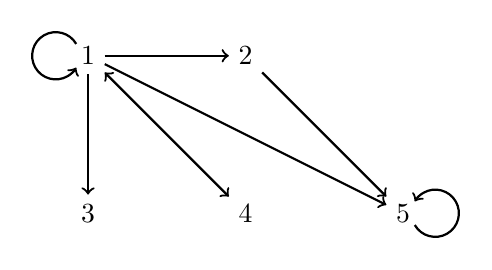
\begin{tikzpicture}
\node (atom1) at (0,2) {1};
\node (atom2) at (2,2) {2};
\node (atom4) at (0,0) {3};
\node (atom5) at (2,0) {4};
\node (atom6) at (4,0) {5};
\draw[->, thick] (atom1)+(-0.15,0.15) arc (-330:-30:.3); 
\draw[->, thick] (atom6)+(0.15,-0.15) arc (-150:150:.3); 
\draw[->, thick] (atom1) -- (atom2);
\draw[->, thick] (atom1) -- (atom4);
\draw[<->, thick] (atom1) -- (atom5);
\draw[->, thick] (atom1) -- (atom6);
\draw[->, thick] (atom2) -- (atom6);
\end{tikzpicture}
\end{center}
Determine whether each of the following sentences is true or false in that interpretation:
\begin{earg}
\item $\exists x\,\atom{R}{x,x}$ \hfill \myanswer{True}
\item $\forall x\,\atom{R}{x,x}$ \hfill \myanswer{False}
\item $\exists x \forall y\,\atom{R}{x,y}$ \hfill \myanswer{True}
\item $\exists x \forall y\,\atom{R}{y,x}$ \hfill \myanswer{False}
\item $\forall x \forall y \forall z ((\atom{R}{x,y} \eand \atom{R}{y,z}) \eif \atom{R}{x,z})$ \hfill \myanswer{False}
\item $\forall x \forall y \forall z ((\atom{R}{x,y} \eand \atom{R}{x,z}) \eif \atom{R}{y,z})$ \hfill \myanswer{False}
\item $\exists x \forall y \enot \atom{R}{x,y}$ \hfill \myanswer{True}
\item $\forall x(\exists y\,\atom{R}{x,y} \eif \exists y\,\atom{R}{y,x})$ \hfill \myanswer{True}
\item $\exists x \exists y (\enot x = y \eand \atom{R}{x,y} \eand \atom{R}{y,x})$ \hfill \myanswer{True}
\item $\exists x \forall y(\atom{R}{x,y} \eiff x = y)$ \hfill \myanswer{True}
\item $\exists x \forall y(\atom{R}{y,x} \eiff x = y)$ \hfill \myanswer{False}
\item $\exists x \exists y(\enot x = y \eand \atom{R}{x,y} \eand \forall z(\atom{R}{z,x} \eiff y = z))$ \hfill \myanswer{True}
\end{earg}
\end{practiceproblems}

\chapter{Semantic concepts}

Offering a precise definition of truth in FOL was more than a little fiddly, but now that we are done, we can define various central logical notions. These will look very similar to the definitions we offered for TFL. However, remember that they concern \emph{interpretations}, rather than valuations.

%We will use the symbol $\entails$ for FOL much as we did for TFL. So:
\factoidbox{
	$$\metaX_1, \metaX_2, \ldots, \metaX_n \therefore\metaZ$$ is \define{valid}
iff there is no interpretation in which all of $\metaX_1, \metaX_2, \ldots, \metaX_n$ are true and in which \metaZ is false. }
%Derivatively,
%	$$\entails\metaX$$
%means that \metaX is true in every interpretation.

The other logical notions also have corresponding definitions in FOL:
\factoidbox{
\begin{itemize}
\item An FOL sentence $\metaX$ is a \define{logical truth} iff $\metaX$ is true in every interpretation.%; i.e.,  $\entails\metaX$.
\newglossaryentry{logical truth}
{
name=logical truth,
description={A \gls{sentence of FOL} that is true in every \gls{interpretation}. Note that the equivalent notion for TFL is `tautology'}
}

\item $\metaX$ is a \define{contradiction} iff $\metaX$ is false in every interpretation.%; i.e., $\entails\enot\metaX$.
\newglossaryentry{contradiction of FOL}
{
  name=contradiction (of FOL),
  text=contradiction,
description={A \gls{sentence of FOL} that is false in every \gls{interpretation}}
}

%\item $\metaX_1, \metaX_2, \ldots \metaX_n \therefore \metaZ$ is \define{valid in FOL} iff there is no interpretation in which all of the premises are true and the conclusion is false; i.e., $\metaX_1,\metaX_2,\ldots \metaX_n \entails\metaZ$. It is \define{invalid in FOL} otherwise.
%\newglossaryentry{logically valid in FOL}
%{
%  name=logical validity (in FOL),
%  text = logically valid,
%description={A property held by arguments if and only if no \gls{interpretation} makes all premises true and the conclusion false}
%}

\item Two FOL sentences \metaX and \metaY are \define{logically equivalent} iff they are true in exactly the same interpretations as each other.%r; i.e., both $\metaX\entails\metaY$ and $\metaY\entails\metaX$.

\newglossaryentry{logically equivalent in FOL}
{
  name=logical equivalence (in FOL),
  text = logically equivalent,
description={A property held by pairs of \glspl{sentence of FOL} if and only if the sentences have the same truth value in every \gls{interpretation}.}
}

\item The FOL sentences $\metaX_1,\metaX_2,\ldots, \metaX_n$ are \define{jointly logically consistent} iff there is some interpretation in which all of the sentences are true. They are \define{jointly logically inconsistent} iff there is no such interpretation.
\newglossaryentry{logically consistent in FOL}
{
  name=logical consistency (in FOL),
  text=jointly consistent,
description={A property held by \glspl{sentence of FOL} if and only if some \gls{interpretation} makes all the sentences true}
}
\end{itemize}
}

\chapter{Using interpretations}
\label{sec.UsingModels}

\section{Logical truths and contradictions}
Suppose we want to show that $\exists xAxx \eif Bd$ is \emph{not} a logical truth. This requires showing that the sentence is not true in every interpretation; i.e.,\ that it is false in some interpretation. If we can provide just one interpretation in which the sentence is false, then we will have shown that the sentence is not a logical truth.

In order for $\exists xAxx \eif Bd$ to be false, the antecedent ($\exists x Axx$) must be true, and the consequent ($Bd$) must be false. To construct such an interpretation, we start by specifying a domain. Keeping the domain small makes it easier to specify what the predicates will be true of, so we will start with a domain that has just one member. For concreteness, let's say it is the city of Paris.
	\begin{ekey}
		\item[\text{domain}] Paris
	\end{ekey}
The name $d$ must refer to something in the domain, so we have no option but:
	\begin{ekey}
		\item[d] Paris
	\end{ekey}
Recall that we want $\exists x Axx$ to be true, so we want all members of the domain to be paired with themselves in the extension of $A$. We can just offer:
	\begin{ekey}
		\item[Axy] \gap{x} is identical with \gap{y}
	\end{ekey}
Now $Add$ is true, so it is surely true that $\exists x Axx$. Next, we want $Bd$ to be false, so the referent of $d$ must not be in the extension of $B$. We might simply offer:
	\begin{ekey}
		\item[Bx] \gap{x} is in Germany
	\end{ekey}
Now we have an interpretation where $\exists x Axx$ is true, but where $Bd$ is false. So there is an interpretation where $\exists x Axx \eif Bd$ is false. So $\exists x Axx \eif Bd$ is not a logical truth.

We can just as easily show that $\exists xAxx \eif Bd$ is not a contradiction. We need only specify an interpretation in which $\exists xAxx \eif Bd$ is true; i.e., an interpretation in which either $\exists x Axx$ is false or $Bd$ is true. Here is one:
	\begin{ekey}
		\item[\text{domain}] Paris
		\item[d] Paris
		\item[Axy] \gap{x} is identical with \gap{y}
		\item[Bx] \gap{x} is in France
	\end{ekey}
This shows that there is an interpretation where $\exists xAxx \eif Bd$ is true. So $\exists x Axx \eif Bd$ is not a contradiction.

\section{Logical equivalence}
Suppose we want to show that $\forall x Sx$ and $\exists x Sx$ are not logically equivalent. We need to construct an interpretation in which the two sentences have different truth values; we want one of them to be true and the other to be false. We start by specifying a domain. Again, we make the domain small so that we can specify extensions easily. In this case, we will need at least two objects. (If we chose a domain with only one member, the two sentences would end up with the same truth value. In order to see why, try constructing some partial interpretations with one-member domains.) For concreteness, let's take:
	\begin{ekey}
		\item[\text{domain}] Ornette Coleman, Miles Davis
	\end{ekey}
We can make $\exists x Sx$ true by including something in the extension of $S$, and we can make $\forall x Sx$ false by leaving something out of the extension of $S$. For concreteness we will offer:
	\begin{ekey}
		\item[Sx] \gap{x} plays saxophone
	\end{ekey}
Now $\exists x Sx$ is true, because $Sx$ is true of Ornette Coleman. Slightly more precisely, extend our interpretation by allowing $c$ to name Ornette Coleman.  $Sc$ is true in this extended interpretation, so $\exists x Sx$ was true in the original interpretation. Similarly, $\forall x Sx$ is false, because $Sx$ is false of Miles Davis. Slightly more precisely, extend our interpretation by allowing $d$ to name Miles Davis, and $Sd$ is false in this extended interpretation, so $\forall x Sx$ was false in the original interpretation. We have provided a counter-interpretation to the claim that $\forall x Sx$ and $\exists x Sx$ are logically equivalent.
	\factoidbox{
		To show that $\metaX$ is not a logical truth, it suffices to find an interpretation where $\metaX$ is false.

		To show that $\metaX$ is not a contradiction, it suffices to find an interpretation where $\metaX$ is true.

		To show that $\metaX$ and $\metaY$ are not logically equivalent, it suffices to find an interpretation where one is true and the other is false.
	}

\section{Validity, entailment and consistency}
To test for validity, entailment, or consistency, we typically need to produce interpretations that determine the truth value of several sentences simultaneously.

Consider the following argument in FOL:
$$\exists x(Gx \eif Ga) \therefore \exists x Gx \eif Ga$$
To show that this is invalid, we must make the premise true and the conclusion false. The conclusion is a conditional, so to make it false, the antecedent must be true and the consequent must be false. Clearly, our domain must contain two objects. Let's try:
	\begin{ekey}
		\item[\text{domain}] Karl Marx, Ludwig von Mises
		\item[Gx] \gap{x} hated communism
		\item[a] Karl Marx
	\end{ekey}
Given that Marx wrote \emph{The Communist Manifesto}, $Ga$ is plainly false in this interpretation. But von Mises famously hated communism, so $\exists x Gx$ is true in this interpretation. Hence $\exists x Gx \eif Ga$ is false, as required.

Does this interpretation make the premise true? Yes it does! Note that $Ga \eif Ga$ is true. (Indeed, it is a logical truth.) But then certainly $\exists x (Gx \eif Ga)$ is true, so the premise is true, and the conclusion is false, in this interpretation. The argument is therefore invalid.

In passing, note that we have also shown that $\exists x(Gx \eif Ga)$ does \emph{not} entail $\exists x Gx \eif Ga$. Equally, we have shown that the sentences $\exists x (Gx \eif Ga)$ and $\enot (\exists x Gx \eif Ga)$ are jointly consistent.

Let's consider a second example. Consider:
	$$\forall x \exists y Lxy \therefore \exists y \forall x Lxy$$
Again, we want to show that this is invalid. To do this, we must make the premises true and the conclusion false. Here is a suggestion:
	\begin{ekey}
		\item[\text{domain}] UK citizens currently in a civil partnership with another UK citizen
		\item[Lxy] \gap{x} is in a civil partnership with \gap{y}
	\end{ekey}
The premise is clearly true on this interpretation. Anyone in the domain is a UK citizen in a civil partnership with some other UK citizen. That other citizen will also, then, be in the domain. So for everyone in the domain, there will be someone (else) in the domain with whom they are in a civil partnership. Hence $\forall x \exists y Lxy$ is true. However, the conclusion is clearly false, for that would require that there is some single person who is in a civil partnership with everyone in the domain, and there is no such person, so the argument is invalid. We observe immediately that the sentences $\forall x \exists y Lxy$ and $\enot\exists y \forall x Lxy$ are jointly consistent and that $\forall x \exists y Lxy$ does not entail $\exists y \forall x Lxy$.

For our third example, we'll mix things up a bit. In \S\ref{s:Interpretations}, we described how we can present some interpretations using diagrams. For example:
\begin{center}
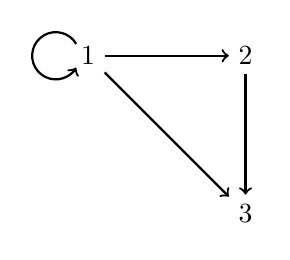
\begin{tikzpicture}
\node (atom1) at (0,2) {1};
\node (atom2) at (2,2) {2};
\node (atom3) at (2,0) {3};
\draw[->, thick] (atom1)--(atom2);
\draw[->, thick] (atom1)--(atom3);
\draw[->, thick] (atom1)+(-0.15,0.15) arc (-330:-30:.3);
\draw[->, thick] (atom2) -- (atom3);
\end{tikzpicture}
\end{center}
Using the conventions employed in \S\ref{s:Interpretations}, the domain of this interpretation is the first three positive whole numbers, and $Rxy$ is true of x and y just in case there is an arrow from x to y in our diagram. Here are some sentences that the interpretation makes true:
	\begin{ebullet}
		\item $\forall x \exists y Ryx$
		\item $\exists x \forall y Rxy$ \hfill witness 1
		\item $\exists x \forall y (Ryx \eiff x = y)$ \hfill witness 1
		\item $\exists x \exists y \exists z ((\enot y = z \eand Rxy) \eand Rzx)$ \hfill witness 2
		\item $\exists x \forall y \enot Rxy$ \hfill witness 3
		\item $\exists x (\exists y Ryx \eand \enot \exists y Rxy)$ \hfill witness 3
	\end{ebullet}
This immediately shows that all of the preceding six sentences are jointly consistent. We can use this observation to generate \emph{invalid} arguments, e.g.:
	\begin{align*}
		\forall x \exists y Ryx, \exists x \forall y Rxy  &\therefore  \forall x \exists y Rxy\\
		\exists x \forall y Rxy, \exists x \forall y \enot Rxy & \therefore \enot \exists x \exists y \exists z (\enot y = z \eand (Rxy \eand Rzx))
	\end{align*}
and many more besides.

	\factoidbox{
	To show that $\metaX_1, \metaX_2, \ldots, \metaX_n \therefore \metaZ$ is invalid, it suffices to find an interpretation where all of $\metaX_1, \metaX_2, \ldots, \metaX_n$ are true and where $\metaZ$ is false.

	That same interpretation will show that $\metaX_1, \metaX_2, \ldots, \metaX_n$ do not entail $\metaZ$.

	It will also show that $\metaX_1, \metaX_2, \ldots, \metaX_n, \enot \metaZ$ are jointly consistent.}
When you provide an interpretation to refute a claim---to logical truth, say, or to entailment---this is sometimes called providing a \emph{counter-interpretation} (or providing a \emph{counter-model}).

\begin{practiceproblems}
\problempart
\label{pr.Contingent}
Show that each of the following is neither a validity nor a contradiction:
\begin{earg}
\item $\atom{D}{a} \eand \atom{D}{b}$

\myanswer{The sentence is true in this model:
\begin{ekey}
	\item[\text{domain}] Stan
	\item[D(x)] Stan
	\item[a] Stan
	\item[b] Stan
\end{ekey}
And it is false in this model:
\begin{ekey}
	\item[\text{domain}] Stan
	\item[D(x)] % $\emptyset$
	\item[a] Stan
	\item[b] Stan
\end{ekey}}
\item \leftsolutions\ $\exists x\,\atom{T}{x,h}$

\myanswer{The sentence is true in this model:
\begin{ekey}
	\item[\text{domain}] Stan
	\item[T(x,y)] \ntuple{Stan, Stan}
	\item[h] Stan
\end{ekey}
And it is false in this model:
\begin{ekey}
	\item[\text{domain}] Stan
	\item[T(x,y)] % $\emptyset$
	\item[h] Stan
\end{ekey}}

\item $\atom{P}{m} \eand \enot\forall x\,\atom{P}{x}$

\myanswer{	The sentence is true in this model:
\begin{ekey}
	\item[\text{domain}] Stan, Ollie
	\item[P(x)] Stan
	\item[m] Stan
\end{ekey}
And it is false in this model:
\begin{ekey}
	\item[\text{domain}] Stan
	\item[P(x)] % $\emptyset$
	\item[m] Stan
\end{ekey}}
\item $\forall z\, \atom{J}{z} \eiff \exists y\,\atom{J}{y}$
\item $\forall x (\atom{W}{x,m,n} \eor \exists y\atom{L}{x,y})$
\item $\exists x (\atom{G}{x} \eif \forall y\,\atom{M}{y})$
\item $\exists x (x = h \eand x = i)$
\end{earg}

\solutions
\problempart
\label{pr.NotEquiv}
Show that the following pairs of sentences are not logically equivalent.
\begin{earg}
\item $\atom{J}{a}$, $\atom{K}{a}$

\myanswer{Making the first sentence true and the second false:
\begin{ekey}
	\item[\text{domain}] $0$
	\item[J(x)] $0$
	\item[K(x)] % $\emptyset$
	\item[a] $0$
\end{ekey}}
\item $\exists x\,\atom{J}{x}$, $\atom{J}{m}$

\myanswer{Making the first sentence true and the second false:
\begin{ekey}
	\item[\text{domain}] $0$, $1$
	\item[J(x)] $0$
	\item[m] $1$
\end{ekey}}
\item $\forall x\,\atom{R}{x,x}$, $\exists x\,\atom{R}{x,x}$

\myanswer{Making the first sentence false and the second true:
\begin{ekey}
	\item[\text{domain}] $0$, $1$
	\item[R(x,y)] \ntuple{$0$,$0$}
\end{ekey}}
\item $\exists x\,\atom{P}{x} \eif \atom{Q}{c}$, $\exists x (\atom{P}{x} \eif \atom{Q}{c})$

\myanswer{Making the first sentence false and the second true:
\begin{ekey}
	\item[\text{domain}] $0$, $1$
	\item[P(x)] $0$
	\item[Q(x)] % $\emptyset$
	\item[c] $0$
\end{ekey}}
\item $\forall x(\atom{P}{x} \eif \enot \atom{Q}{x})$, $\exists x(\atom{P}{x} \eand \enot \atom{Q}{x})$

\myanswer{Making the first sentence true and the second false:
\begin{ekey}
	\item[\text{domain}] $0$
	\item[P(x)] % $\emptyset$
	\item[Q(x)] % $\emptyset$
\end{ekey}}
\item $\exists x(\atom{P}{x} \eand \atom{Q}{x})$, $\exists x(\atom{P}{x} \eif \atom{Q}{x})$

\myanswer{Making the first sentence false and the second true:
\begin{ekey}
	\item[\text{domain}] $0$
	\item[P(x)] % $\emptyset$
	\item[Q(x)] $0$
\end{ekey}}
\item $\forall x(\atom{P}{x}\eif \atom{Q}{x})$, $\forall x(\atom{P}{x} \eand \atom{Q}{x})$

\myanswer{Making the first sentence true and the second false:
\begin{ekey}
	\item[\text{domain}] $0$
	\item[P(x)] % $\emptyset$
	\item[Q(x)] $0$
\end{ekey}}
\item $\forall x\exists y\,\atom{R}{x,y}$, $\exists x\forall y\,\atom{R}{x,y}$

\myanswer{Making the first sentence true and the second false:
\begin{ekey}
	\item[\text{domain}] $0$, $1$
	\item[R(x,y)] \ntuple{$0$, $1$}, \ntuple{$1$, $0$}
\end{ekey}}
\item $\forall x\exists y\,\atom{R}{x,y}$, $\forall x\exists y\,\atom{R}{y,x}$

\myanswer{Making the first sentence false and the second true:
\begin{ekey}
	\item[\text{domain}] $0$, $1$
	\item[R(x,y)] \ntuple{$0$, $0$}, \ntuple{$0$, $1$}
\end{ekey}}
\end{earg}


\problempart
Show that the following sentences are jointly satisfiable:
\begin{earg}
\item $\atom{M}{a}, \enot \atom{N}{a}, Pa, \enot \atom{Q}{a}$
\item $\atom{L}{e,e}, \atom{L}{e,g}, \enot \atom{L}{g,e}, \enot \atom{L}{g,g}$
\item $\enot (\atom{M}{a} \eand \exists x\,\atom{A}{x}), Ma \eor \atom{F}{a}, \forall x(\atom{F}{x} \eif \atom{A}{x})$
\item $\atom{M}{a} \eor \atom{M}{b}, \atom{M}{a} \eif \forall x \enot \atom{M}{x}$
\item $\forall y\,\atom{G}{y}, \forall x (\atom{G}{x} \eif \atom{H}{x}), \exists y \enot \atom{I}{y}$
\item $\exists x(\atom{B}{x} \eor \atom{A}{x}), \forall x \enot \atom{C}{x}, \forall x\bigl[(\atom{A}{x} \eand \atom{B}{x}) \eif Cx\bigr]$
\item $\exists x\,\atom{X}{x}, \exists x\,\atom{Y}{x}, \forall x(\atom{X}{x} \eiff \enot \atom{Y}{x})$
\item $\forall x(\atom{P}{x} \eor \atom{Q}{x}), \exists x\enot(\atom{Q}{x} \eand \atom{P}{x})$
\item $\exists z(\atom{N}{z} \eand \atom{O}{z,z}), \forall x\forall y(\atom{O}{x,y} \eif \atom{O}{y,x})$
\item $\enot \exists x \forall y\,\atom{R}{x,y}, \forall x \exists y\,\atom{R}{x,y}$
\item $\enot \atom{R}{a,a}$, $\forall x (x=a \eor \atom{R}{x,a})$

\myanswer{The sentences are both true in this interpretation:
\begin{ekey}
	\item[\text{domain}] Harry, Sally
	\item[R(x,y)]\ntuple{Sally, Harry}
	\item[a] Harry
	\end{ekey}}
\item $\forall x\forall y\forall z[(x=y \eor y=z )\eor x=z]$, $\exists x\exists y\ \enot x= y$

\myanswer{There are no predicates or constants, so we only need to give a domain.
Any domain with 2 elements will do.}
\item $\exists x\exists y((\atom{Z}{x} \eand \atom{Z}{y} )\eand x=y)$, $\enot \atom{Z}{d}$, $d=e$
\end{earg}

\problempart
Show that the following arguments are invalid:
\begin{earg}
\item $\forall x(\atom{A}{x} \eif \atom{B}{x}) \therefore \exists x\,\atom{B}{x}$
\item $\forall x(\atom{R}{x} \eif \atom{D}{x}), \forall x(\atom{R}{x} \eif \atom{F}{x}) \therefore \exists x(\atom{D}{x} \eand \atom{F}{x})$
\item $\exists x(\atom{P}{x}\eif \atom{Q}{x}) \therefore \exists x\,\atom{P}{x}$
\item $\atom{N}{a} \eand \atom{N}{b} \eand \atom{N}{c} \therefore \forall x\,\atom{N}{x}$
\item $\atom{R}{d,e}, \exists x\,\atom{R}{xd} \therefore \atom{R}{e,d}$
\item $\exists x(\atom{E}{x} \eand \atom{F}{x}), \exists x\,\atom{F}{x} \eif \exists x\,\atom{G}{x} \therefore \exists x(\atom{E}{x} \eand \atom{G}{x})$
\item $\forall x\,\atom{O}{x,c}, \forall x\,\atom{O}{c,x} \therefore \forall x\,\atom{O}{x,x}$
\item $\exists x(\atom{J}{x} \eand \atom{K}{x}), \exists x \enot \atom{K}{x}, \exists x \enot \atom{J}{x} \therefore \exists x(\enot \atom{J}{x} \eand \enot \atom{K}{x})$
\item $\atom{L}{a,b} \eif \forall x\,\atom{L}{x,b}, \exists x\,\atom{L}{x,b} \therefore \atom{L}{b,b}$
\item $\forall x(\atom{D}{x} \eif \exists y\,\atom{T}{y,x}) \therefore \exists y \exists z\ \enot y= z$
\end{earg}


\end{practiceproblems}


\chapter{Reasoning about all interpretations}

\section{Logical truths and contradictions}
We can show that a sentence is \emph{not} a logical truth just by providing one carefully specified interpretation: an interpretation in which the sentence is false. To show that something is a logical truth, on the other hand, it would not be enough to construct ten, one hundred, or even a thousand interpretations in which the sentence is true. A sentence is only a logical truth if it is true in \emph{every} interpretation, and there are infinitely many interpretations. We need to reason about all of them, and we cannot do this by dealing with them one by one!

Sometimes, we can reason about all interpretations fairly easily. For example, we can offer a relatively simple argument that $Raa\eiff Raa$ is a logical truth:
	\begin{quote}
		\label{allmodels1}
		Any relevant interpretation will give $Raa$ a truth value. If $Raa$ is true in an interpretation, then $Raa \eiff Raa$ is true in that interpretation. If $Raa$ is false in an interpretation, then $Raa \eiff Raa$ is true in that interpretation. These are the only alternatives. So $Raa \eiff Raa$ is true in every interpretation. Therefore, it is a logical truth.
	\end{quote}
This argument is valid, of course, and its conclusion is true. However, it is not an argument in FOL. Rather, it is an argument in English \emph{about} FOL: it is an argument in the metalanguage.

Note another feature of the argument. Since the sentence in question contained no quantifiers, we did not need to think about how to interpret $a$ and $R$; the point was just that, however we interpreted them, $Raa$ would have some truth value or other. (We could ultimately have given the same argument concerning TFL sentences.)

Here is another bit of reasoning. Consider the sentence $\forall x(Rxx\eiff Rxx)$. Again, it should obviously be a logical truth, but to say precisely why is quite a challenge. We cannot say that $Rxx \eiff Rxx$ is true in every interpretation, since $Rxx \eiff Rxx$ is not even a \emph{sentence} of FOL (remember that $x$ is a variable, not a name). So we have to be a bit cleverer.
	\begin{quote}
		Consider some arbitrary interpretation. Consider some arbitrary member of the domain, which, for convenience, we will call \emph{obbie}, and suppose we extend our original interpretation by adding a new name, $c$, to name \emph{obbie}. Then either $Rcc$ will be true or it will be false. If $Rcc$ is true, then $Rcc \eiff Rcc$ is true. If $Rcc$ is false, then $Rcc \eiff Rcc$ will be true. So either way, $Rcc \eiff Rcc$ is true. Since there was nothing special about \emph{obbie}---we might have chosen any object---we see that no matter how we extend our original interpretation by allowing $c$ to name some new object, $Rcc \eiff Rcc$ will be true in the new interpretation. So $\forall x (Rxx \eiff Rxx)$ was true in the original interpretation. But we chose our interpretation arbitrarily, so $\forall x (Rxx \eiff Rxx)$ is true in every interpretation. It is therefore a logical truth.
	\end{quote}
This is quite longwinded, but, as things stand, there is no alternative. In order to show that a sentence is a logical truth, we must reason about \emph{all} interpretations.

\section{Other cases}
Similar points hold of other cases too. Thus, we must reason about all interpretations if we want to show:
	\begin{ebullet}
		\item that a sentence is a contradiction; for this requires that it is false in \emph{every} interpretation.
		\item that two sentences are logically equivalent; for this requires that they have the same truth value in \emph{every} interpretation.
		\item that some sentences are jointly inconsistent; for this requires that there is no interpretation in which all of those sentences are true together; i.e.\ that, in \emph{every} interpretation, at  least one of those sentences is false.
		\item that an argument is valid; for this requires that the conclusion is true in \emph{every} interpretation where the premises are true.
		\item that some sentences entail another sentence.
	\end{ebullet}
The problem is that, with the tools available to you so far, reasoning about all interpretations is a serious challenge! Let's take just one more example. Here is an argument which is obviously valid:
	$$\forall x(Hx \eand Jx) \therefore \forall x Hx$$
After all, if everything is both H and J, then everything is H. But we can only show that the argument is valid by considering what must be true in every interpretation in which the premise is true. To show this, we would have to reason as follows:
	\begin{quote}
		Consider an arbitrary interpretation in which the premise $\forall x(Hx \eand Jx)$ is true. It follows that, however we expand the interpretation with a new name, for example $c$, $Hc \eand Jc$ will be true in this new interpretation. $Hc$ will, then, also be true in this new interpretation. But since this held for \emph{any} way of expanding the interpretation, it must be that $\forall x Hx$ is true in the old interpretation. We've assumed nothing about the interpretation except that it was one in which $\forall x(Hx \eand Jx)$  is true, so any interpretation in which $\forall x(Hx \eand Jx)$ is true is one in which $\forall x Hx$ is true. The argument is valid!
\end{quote}
Even for a simple argument like this one, the reasoning is somewhat complicated. For longer arguments, the reasoning can be extremely torturous.

The following table summarises whether a single (counter-)interpretation suffices, or whether we must reason about all interpretations.


\begin{center}
\begin{tabular}{l l l}
%\cline{2-3}
 & \textbf{Yes} & \textbf{No}\\
 \hline
%\cline{2-3}
logical truth? & all interpretations & one counter-interpretation\\
contradiction? &  all interpretations  & one counter-interpretation\\
equivalent? & all interpretations & one counter-interpretation\\
consistent? & one interpretation & all interpretations\\
valid? & all interpretations & one counter-interpretation\\
entailment? & all interpretations & one counter-interpretation\\
\end{tabular}
\end{center}
\label{table.ModelOrArgument}

This might usefully be compared with the table at the end of \S\ref{s:PartialTruthTable}. The key difference resides in the fact that TFL concerns truth tables, whereas FOL concerns interpretations. This difference is deeply important, since each truth-table only ever has finitely many lines, so that a complete truth table is a relatively tractable object. By contrast, there are infinitely many interpretations for any given sentence(s), so that reasoning about all interpretations can be a deeply tricky business.
